\documentclass{exam}
%\documentclass[11pt,a4paper]{exam}
\usepackage{amsmath,amsthm,amsfonts,amssymb,dsfont}
\usepackage{ifthen}
\usepackage[legalpaper, total={177.8mm, 290mm}]{geometry}
\usepackage{enumerate}% http://ctan.org/pkg/enumerate
\usepackage{multicol}
\usepackage{hhline}
\usepackage[table]{xcolor}
\usepackage{graphicx}


% Accumulate the answers. Unmodified from Phil Hirschorn's answer
% https://tex.stackexchange.com/questions/15350/showing-solutions-of-the-questions-separately/15353
\newbox\allanswers
\setbox\allanswers=\vbox{}

\newenvironment{answer}
{%
    \global\setbox\allanswers=\vbox\bgroup
    \unvbox\allanswers
}%
{%
    \bigbreak
    \egroup
}

\newcommand{\showallanswers}{\par\unvbox\allanswers}
% End Phil's answer


% Is there a better way?
\newcommand*{\getanswer}[5]{%
    \ifthenelse{\equal{#5}{a}}
    {\begin{answer}\thequestion. (a)~#1\end{answer}}
    {\ifthenelse{\equal{#5}{b}}
        {\begin{answer}\thequestion. (b)~#2\end{answer}}
        {\ifthenelse{\equal{#5}{c}}
            {\begin{answer}\thequestion. (c)~#3\end{answer}}
            {\ifthenelse{\equal{#5}{d}}
                {\begin{answer}\thequestion. (d)~#4\end{answer}}
                {\begin{answer}\textbf{\thequestion. (#5)~Invalid answer choice.}\end{answer}}}}}
}

\setlength\parindent{0pt}
%usage \choice{ }{ }{ }{ }
%(A)(B)(C)(D)
\newcommand{\fourch}[5]{
    \par
    \begin{tabular}{*{4}{@{}p{0.23\textwidth}}}
        (a)~#1 & (b)~#2 & (c)~#3 & (d)~#4
    \end{tabular}
    \getanswer{#1}{#2}{#3}{#4}{#5}
}

%(A)(B)
%(C)(D)
\newcommand{\twoch}[5]{
    \par
    \begin{tabular}{*{2}{@{}p{0.46\textwidth}}}
        (a)~#1 & (b)~#2
    \end{tabular}
    \par
    \begin{tabular}{*{2}{@{}p{0.46\textwidth}}}
        (c)~#3 & (d)~#4
    \end{tabular}
    \getanswer{#1}{#2}{#3}{#4}{#5}
}

%(A)
%(B)
%(C)
%(D)
\newcommand{\onech}[5]{
    \par
    (a)~#1 \par (b)~#2 \par (c)~#3 \par (d)~#4
    \getanswer{#1}{#2}{#3}{#4}{#5}
}

\newlength\widthcha
\newlength\widthchb
\newlength\widthchc
\newlength\widthchd
\newlength\widthch
\newlength\tabmaxwidth

\setlength\tabmaxwidth{0.96\textwidth}
\newlength\fourthtabwidth
\setlength\fourthtabwidth{0.25\textwidth}
\newlength\halftabwidth
\setlength\halftabwidth{0.5\textwidth}

\newcommand{\choice}[5]{%
\settowidth\widthcha{AM.#1}\setlength{\widthch}{\widthcha}%
\settowidth\widthchb{BM.#2}%
\ifdim\widthch<\widthchb\relax\setlength{\widthch}{\widthchb}\fi%
    \settowidth\widthchb{CM.#3}%
\ifdim\widthch<\widthchb\relax\setlength{\widthch}{\widthchb}\fi%
    \settowidth\widthchb{DM.#4}%
\ifdim\widthch<\widthchb\relax\setlength{\widthch}{\widthchb}\fi%

% These if statements were bypassing the \onech option.
% \ifdim\widthch<\fourthtabwidth
%     \fourch{#1}{#2}{#3}{#4}{#5}
% \else\ifdim\widthch<\halftabwidth
% \ifdim\widthch>\fourthtabwidth
%     \twoch{#1}{#2}{#3}{#4}{#5}
% \else
%      \onech{#1}{#2}{#3}{#4}{#5}
%  \fi\fi\fi}

% Allows for the \onech option.
\ifdim\widthch>\halftabwidth
    \onech{#1}{#2}{#3}{#4}{#5}
\else\ifdim\widthch<\halftabwidth
\ifdim\widthch>\fourthtabwidth
    \twoch{#1}{#2}{#3}{#4}{#5}
\else
    \fourch{#1}{#2}{#3}{#4}{#5}
\fi\fi\fi}


\begin{document}

\begin{table}[h]
\centering
\begin{tabular}{lllll}
\textbf{\large SYLHET CADET COLLEGE} &  &  &  &  \\ \cline{4-5} 
PROGRESS TEST EXAMINATION - 2024 &  & \multicolumn{1}{l|}{} & \multicolumn{1}{l|}{Set} & \multicolumn{1}{l|}{:A} \\ \cline{4-5} 
CLASS: XI &  &  &  &  \\ \cline{3-5} 
MULTIPLE CHOICE QUESTIONS & \multicolumn{1}{l|}{\textbf{Subject Code:}} & \multicolumn{1}{l|}{1} & \multicolumn{1}{l|}{2} & \multicolumn{1}{l|}{9} \\ \cline{3-5} 
STATISTICS FIRST PAPER &  &  &  &  \\
TIME – 25 minutes &  &  &  &  \\
FULL MARKS – 25 &  &  &  & 
\end{tabular}
\end{table}
%  \normalfont\normalsize
 % 11.45a.m.~--~1.45p.m.
\hrule

\begin{center}
[N.B. – Answer all the questions. Each question carries ONE mark. Block fully, with a black ball- point pen, the circle of the letter that stands for the correct/best answer in the “Answer sheet” for the Multiple Choice Questions Examination.]\\

  
  \textbf{Candidates are asked not to leave any mark or spot on the question paper.}
\end{center}
\begin{questions}


\question \textbf{A researcher collected data on age and income of the people in a city. The variables are --}

i. bi-variate \\
ii. quantitative \\
iii. qualitative

\textbf{Which one is correct?}

\choice{i and ii}{i and iii}{ii and iii}{i, ii and iii}{a}

\question \textbf{Which measurement scale does height belong to?}
\choice{Nominal}{Ordinal}{Interval}{Ratio}{d}

\question \textbf{The arithmetic mean of first 10 natural numbers is:}
\choice{6}{8.5}{5.5}{5.6}{c}

\question \textbf{If a data set is divided into five parts, how many partition values are created?}
\choice{4}{5}{6}{3}{a}

\question \textbf{When is the statement $AM=GM=HM$ true?}
\choice{When the values are natural numbers}{When all the values are equal}{When all the values have equal frequency}{When mode is greater than median}{a}

\question \textbf{Which is considered statistics?}
\choice{Jaman obtain 75 in statistics}{Shafiq lives at Road no. 5}{Mean monthly income in a city is 60,000 taka}{Width of a book is 10 cm}{c}


\question \textbf{$If x_1=2, x_2=3, x_3=4, x_4=6$, and $x_5=5, \displaystyle \sum_{i=1}^4 x_i^2=?$}
\choice{80}{87}{90}{105}{c}

\question \textbf{Which can be measured from the Ogive?}
\choice{Arithmetic Mean}{Geometric Mean}{Median}{Mode}{c}

\textbf{Answer the next three questions based on the following information}

\begin{center}
The data collected in a research is this: 1, 2, 4, 8, 16, 32
\end{center}

\question \textbf{Which measure is suitable?}
\choice{Arithmetic Mean}{Geometric Mean}{Median}{Mode}{b}

\question \textbf{What is the arithmetic mean of the data?}
\choice{8.5}{10}{8}{10.5}{d}

\question \textbf{What is the geometric mean?}
\choice{8.5}{5.66}{6.55}{16}{b}

\question \textbf{The arithmetic mean and geometric mean of two non-zero positive numbers are 15 and 10, respectively. What is harmonic mean?}
\choice{6.61}{6.67}{7.66}{6.76}{b}

\question \textbf{A good measure of central tendency -}

i. is loosly defined \\
ii. takes into consideration all values \\
iii. easily understandable

\textbf{Which one is correct?}

\choice{i and ii}{i and iii}{ii and iii}{i, ii and iii}{c}

\question \textbf{What is the harmonic mean of these values: 10, 12, 13, 15, 20, 25}
\choice{12.49}{14.93}{14.39}{13.49}{c}

\question \textbf{What is true of harmonic mean?}

i. uses all values in tha data \\
ii. undefined if the any value is zero \\
iii. affected by extreme values

\textbf{Which one is correct?}

\choice{i and ii}{i and iii}{ii and iii}{i, ii and iii}{a}

\question \textbf{What is formula of rth raw moment for grouped data about a?}
\choice{$\frac{\sum f_i(x_i-a)^r}{n}$}{$\frac{\sum f_i(x_i-\bar x)^r}{n}$}{$\frac{\sum (x_i-a)^r}{n}$}{$\frac{\sum (x_i+a)^r}{n}$}{a}

\question \textbf{Which relatonship is correct?}
\choice{$\mu_1' = \bar x + a$}{$\mu_1' = \bar x - a$}{$\mu_2' = \bar x + a$}{$\mu_1 = \bar x - a$}{b}

\question \textbf{If $\gamma_1 > 0$, the data is -}
\choice{Negatively skewed}{Positively skewed}{Symmetric}{Uncertain}{b}

\question \textbf{Which relationship is correct?}
\choice{$M_o = 2Me - \bar x$}{$M_o = 3Me - \bar x$}{$M_o = 3Me - 2 \bar x$}{$M_o = 2Me - 3 \bar x$}{a}

\question \textbf{Which curve is platykurtic?}

\begin{center}
   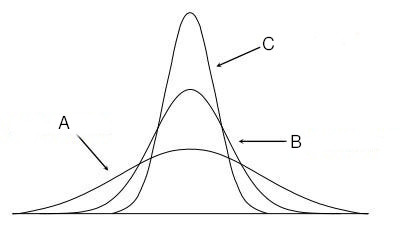
\includegraphics[width=0.4\textwidth]{../img/kurtosis.jpg}
\end{center}

\choice{A}{B}{C}{None}{a}

\question \textbf{What is formula of the left inner fence for a box and whisker plot?}
\choice{$Q_1-1.5 \times IQR$}{$Q_3+1.5 \times IQR$}{$Q_1-3 \times IQR$}{$Q_3+1.5 \times IQR$}{a}


%\question \textbf{To complete the song, the last answer should be
%\choice{a}{b}{c}{d}{e} % Invalid answer choice

\end{questions}

 \vspace{2.5cm}

\begin{center}
Figures don't lie, but liars figure.  - Mark Twain
\end{center}

\pagebreak
%\newpage  %Uncomment to put on new age
\bigskip

\begin{multicols}{3}
[
Answer Key
]
\showallanswers % Phil Hirschorn
\end{multicols}


\end{document}